\chapter{Cluster Analysis}
\section{Introduction}
Clustering are a familiy of \textbf{unsupervised learning} problems, where we we want to group objects in non-overlapping subsets, called \textbf{clusters}, according to a criterion of \textit{similarity}.

In other kind of problems, such as classiifcation and regression, we want to minimize the error terms, while in clustering we want to maximize the similarity between the objects in the same cluster.

\callout{Note}{It can be seen as a degenerate case of classification, but we avoid to use the term "classification" because it is usually associated with supervised learning and because in this case we dont'have the same theretical structure.}

\subsubsection*{Role of similarity}
In order to group observations into clusters, it is necessary to define how \textit{similar/dissimilar} they are.

However, there is no universal definition of \textit{similarity}, but it is something that depends on the specific application or subjective criteria, and it also depends on the algorithm we use as it must be applicable.

We can think of the similarity measure as a counterpart of the loss function used in supervised applications.
In fact, if the loss function does not fit the data generation model well, the process will have low performance; likewise, if the similarity measure does not fit the observations we are considering, the analysis will have poor performance.

\subsubsection*{Clustering methods}

There are four main families of clustering:
\begin{itemize}
    \item \textbf{Combinatorial}, where we want to minimize over the set of all possible assigments, a suitable function based on the chosen similarity measure. This is a combinatorial problem since we have a large number of possible assignments.
    \item \textbf{Distribution-based}, where we assume that the data observations have been drawn from a mixture of \textbf{generative models}, and we want to find the parameters of the models. The parameters of the models are estimated from the observation using an \textit{expectation-maximization} algorithm. After the parameters have been estimated, we can assign each observation to a model according to the probability of being generated by one of the models.
    \item \textbf{Hierarchical}, assign each data observation to a cluster according to the similarity among pair of groups of observations. This is done by building a \textit{tree structure} to represent the data. Such structure can be obtained by using a \textit{bottom-up} or \textit{top-down} approach and the algorithms are called respectively \textit{agglomerative} or \textit{divisive} clustering.
    \item \textbf{Density-based}, where clusters follow more closely the spatial arrangement of the data. The clusters are defined as regions with densely packed observation. Density is usually intendend as the number of observations within a given volume.
\end{itemize}

Figure \ref{fig:clustering_methods} shows an example of the different clustering methods.

\begin{figure}
    \centering
    \begin{minipage}{0.45\textwidth}
        \centering
        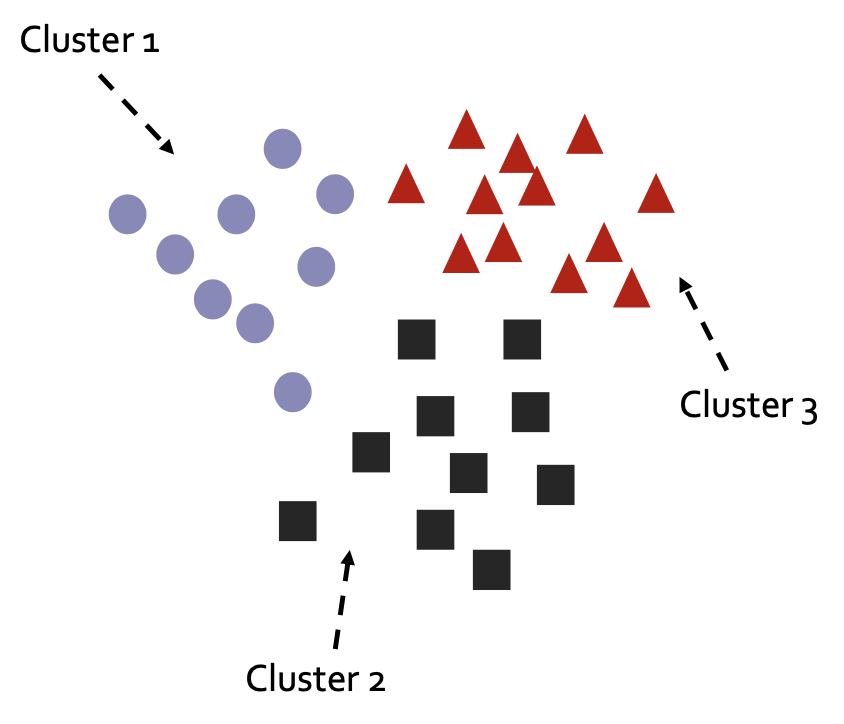
\includegraphics[width=\linewidth]{./figures/chapter_7/combinatorial.png}
        \caption{Combinatorial clustering}
        \label{fig:combex}
    \end{minipage}
    \hfill
    \begin{minipage}{0.45\textwidth}
        \centering
        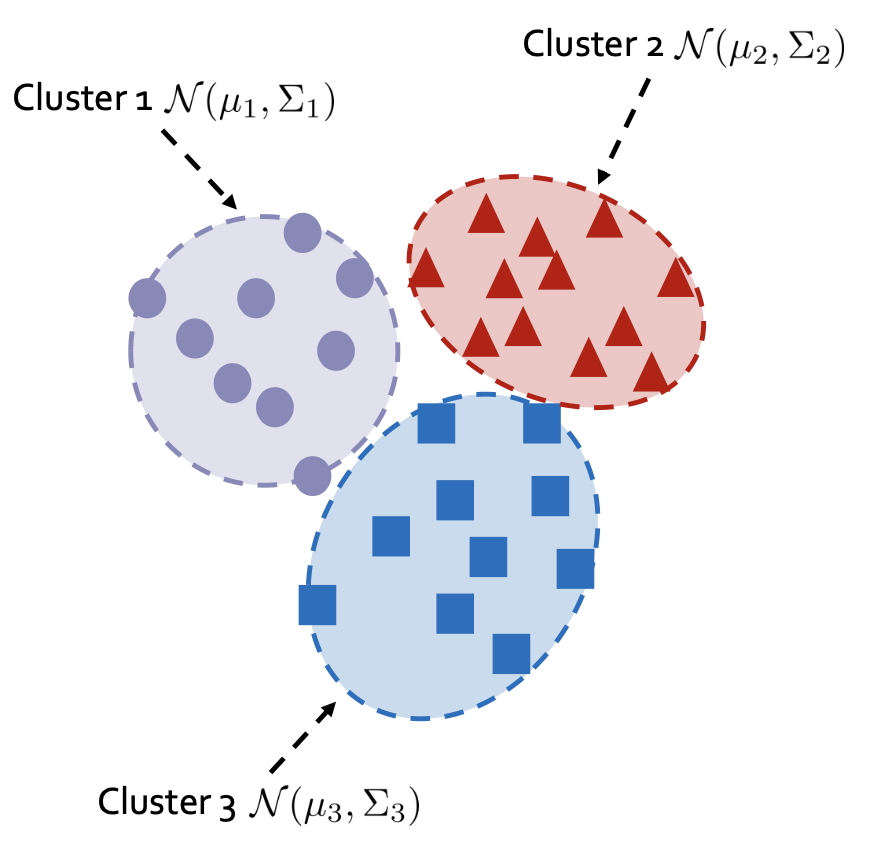
\includegraphics[width=\linewidth]{./figures/chapter_7/distribution.png}
        \caption{Distribution based clustering}
        \label{fig:distribex}
    \end{minipage}
    \vskip\baselineskip
    \begin{minipage}{0.45\textwidth}
        \centering
        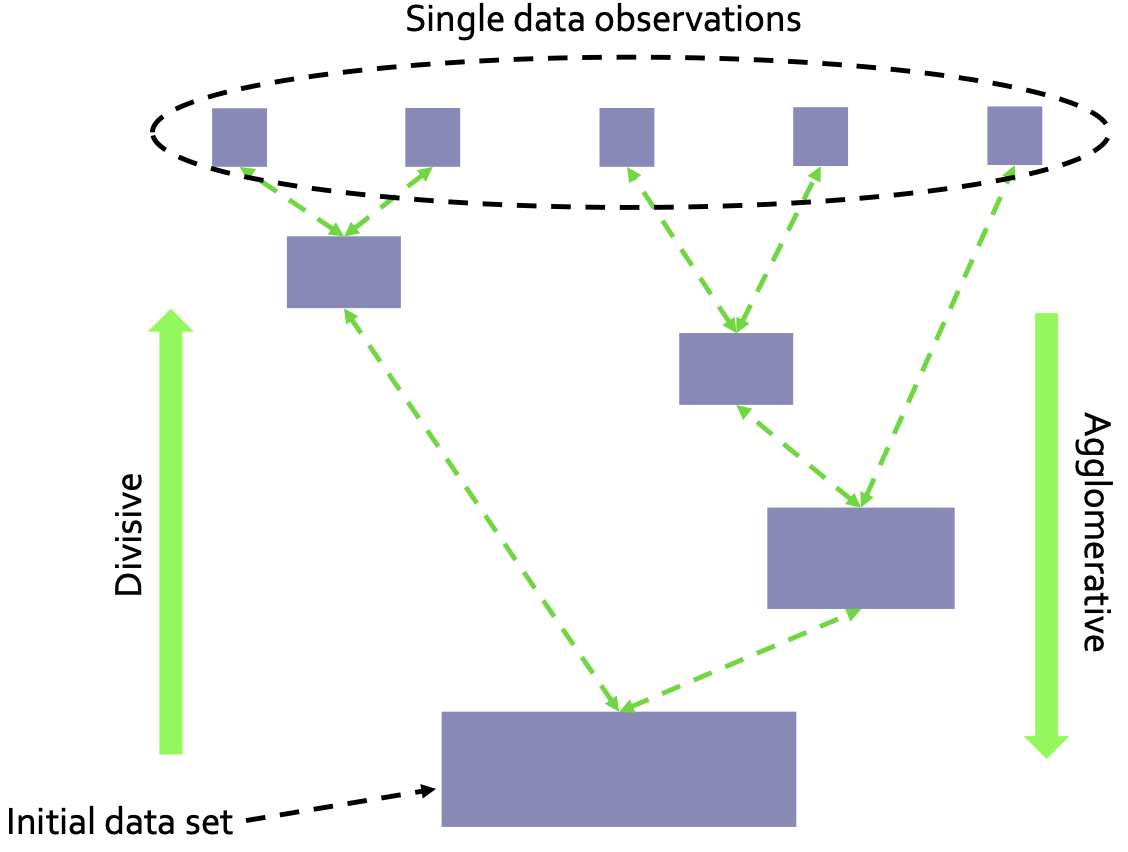
\includegraphics[width=\linewidth]{./figures/chapter_7/hierarchical.png}
        \caption{Hierarchical clustering}
        \label{fig:hierarcex}
    \end{minipage}
    \hfill
    \begin{minipage}{0.45\textwidth}
        \centering
        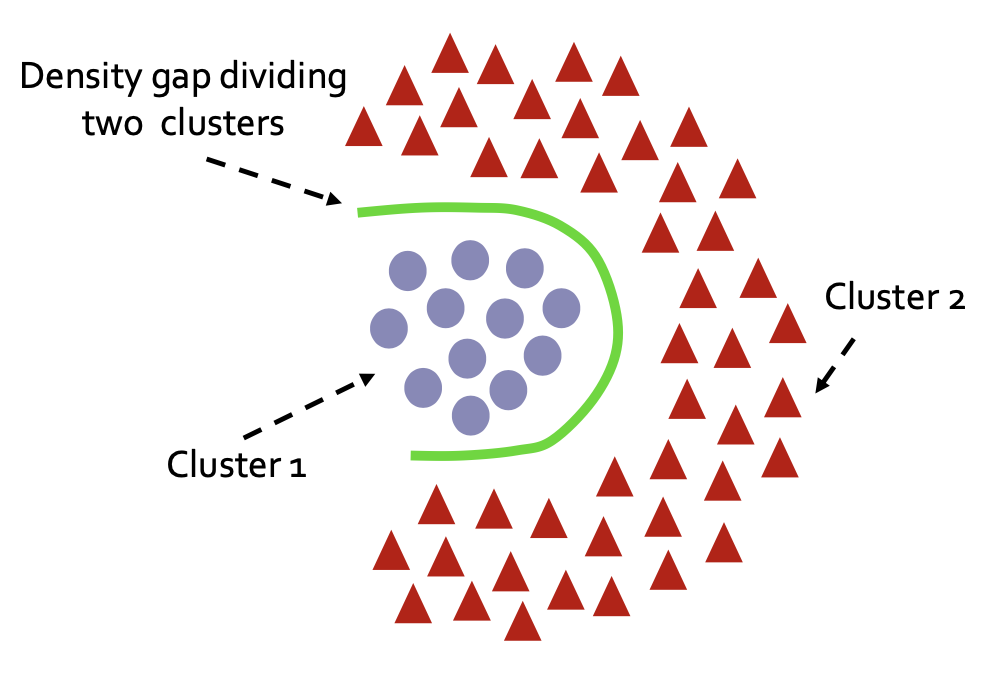
\includegraphics[width=\linewidth]{./figures/chapter_7/density.png}
        \caption{Density-based clustering}
        \label{fig:densityex}
    \end{minipage}
    \caption{Clustering methods example}
    \label{fig:clustering_methods}
\end{figure}


\section{K-Means}
The K-Means algorithm is a combinatorial clustering algorithm.

The number of clusters $K$ is a parameter of the algorithm, and it is usually chosen by the user. The algorithm is iterative and its goal is to find the optimal assigment of the observation that minimizes the following sum of squares:
\[
    J = \sum_{n=1}^{N} \sum_{k=1}^K r_{nk} \|x_n - \mu_k\|^2
\]

Where:
\begin{itemize}
    \item $r_{nk}$ is a variable that is equal to $1$ if the observation $x_n$ is assigned to the cluster $C_k$, and $0$ otherwise
    \item $\mu_k$ is the \textbf{centroid} of the cluster $C_k$, defined as:
    \[
        \mu_k = \frac{\sum_{n=1}^{N} r_{nk} x_n}{\sum_{n=1}^{N} r_{nk}}
    \]
    The centroid can be seen as the \textit{baricenter} of the cluster $C_k$. 
\end{itemize}

Note that we are minimizing a quantity that represents how dispersed the observations are around the centroid of each cluster.

The quantity $J$ considers the distance from a certain observation $x_n$ from the centroid of the cluster $C_k$, in such a way to obtain a measure of the dispersion of the cluster. The centroids are the value that minimizes $J$ for a given fixed assignment $r_{nk}$.

A naïve solution to find the best assigment would be the \textit{exhaustive search} one, described by the following steps:
\begin{algorithm}
    \SetAlgoLined
    \SetKwInOut{Input}{Input}
    \SetKwInOut{Output}{Output}
    
    \Input{Data set $X$, number of clusters $K$}
    \Output{Optimal assignment $r^\ast$}
    
    $J_{\text{min}} \leftarrow \infty$\;
    $r^\ast \leftarrow \emptyset$\;
    
    \For{each possible assignment $r$}{
        Compute the corresponding $J$\;
        
        \If{$J < J_{\text{min}}$}{
            $J_{\text{min}} \leftarrow J$\;
            $r^\ast \leftarrow r$\;
        }
    }
    
    \caption{Exhaustive Search for Optimal Assignment}
\end{algorithm}

The first problem with this approach is that the number of possible assignments is very large, so the algorithm is not feasible in general. 

A better strategy is, given the centroids $\mu_k$, to find the best assigment $r_{nk}$ that minimizes the objective function by using the \textbf{nearest neighbor condition}. That condition states:
\[
    r_{nk} = 1 \text{if } k = \arg\min_{j} \|x_n - \mu_j\|^2 \text{ else } r_{nk} = 0 
\]

There is a problem with this formulation, that is the fact that the centroids are a function of the assigments, but we don't know both of them.
In fact, we've said that they're the minimizer of the objective function given a fixed assignment. And they could be computed as:
\[
    \mu_k = \frac{\sum_{n=1}^{N} r_{nk} x_n}{\sum_{n=1}^{N} r_{nk}}
\]
By the way we are in a \textit{chicken and egg} problem.

There is a problem with this formulation, that is the fact that the centroids are a function of the assigments, but we don't know both of them. So a \textit{naive} solution would be to enumerate both of them and choose the best one, and this is why it is called a combinatorial problem.

% However, we know that given the centroids, the assigments $r_{nk}$ should be:
% \[
%     r_{nk} = 1 \text{if } k = \arg\min_{j} \|x_n - \mu_j\|^2
% \]
% and $0$ otherwise. This is called the \textbf{nearest neighbor condition}. If the assigments follow this rule, this will reduce the objective function. Given the assigments, the centroids can be computed by definition \textbf{centroid condition}.

\subsubsection*{Lloyd's Algorithm}

The solution to the K-Means problem is given by the \textbf{Lloyd's algorithm}, which is an iterative algorithm that alternates between the two steps of finding the best assigment given the centroids and finding the best centroids given the assigments.
That process is repeated until the algorithm converges and so a stop condition is met.

There are several versions of the Lloyd's algorithm that differ on the trade-off between accuracy and efficiency. A pseudo-code of the algorithm is shown in Algorithm \ref{alg:lloyd}.

\begin{algorithm}
    \SetAlgoLined
    Input: data set $X$, number of clusters $K$, initial centroids $\mu_k$ \\
    \Repeat{termination criterion is met}{
        form $K$ clusters assigning each observation to the nearest centroid \\
        recompute the centroids $\mu_k$ of the clusters \\
    }
    \caption{Lloyd's algorithm for K-Means}
    \label{alg:lloyd}
\end{algorithm}

\begin{figure}
    \centering
    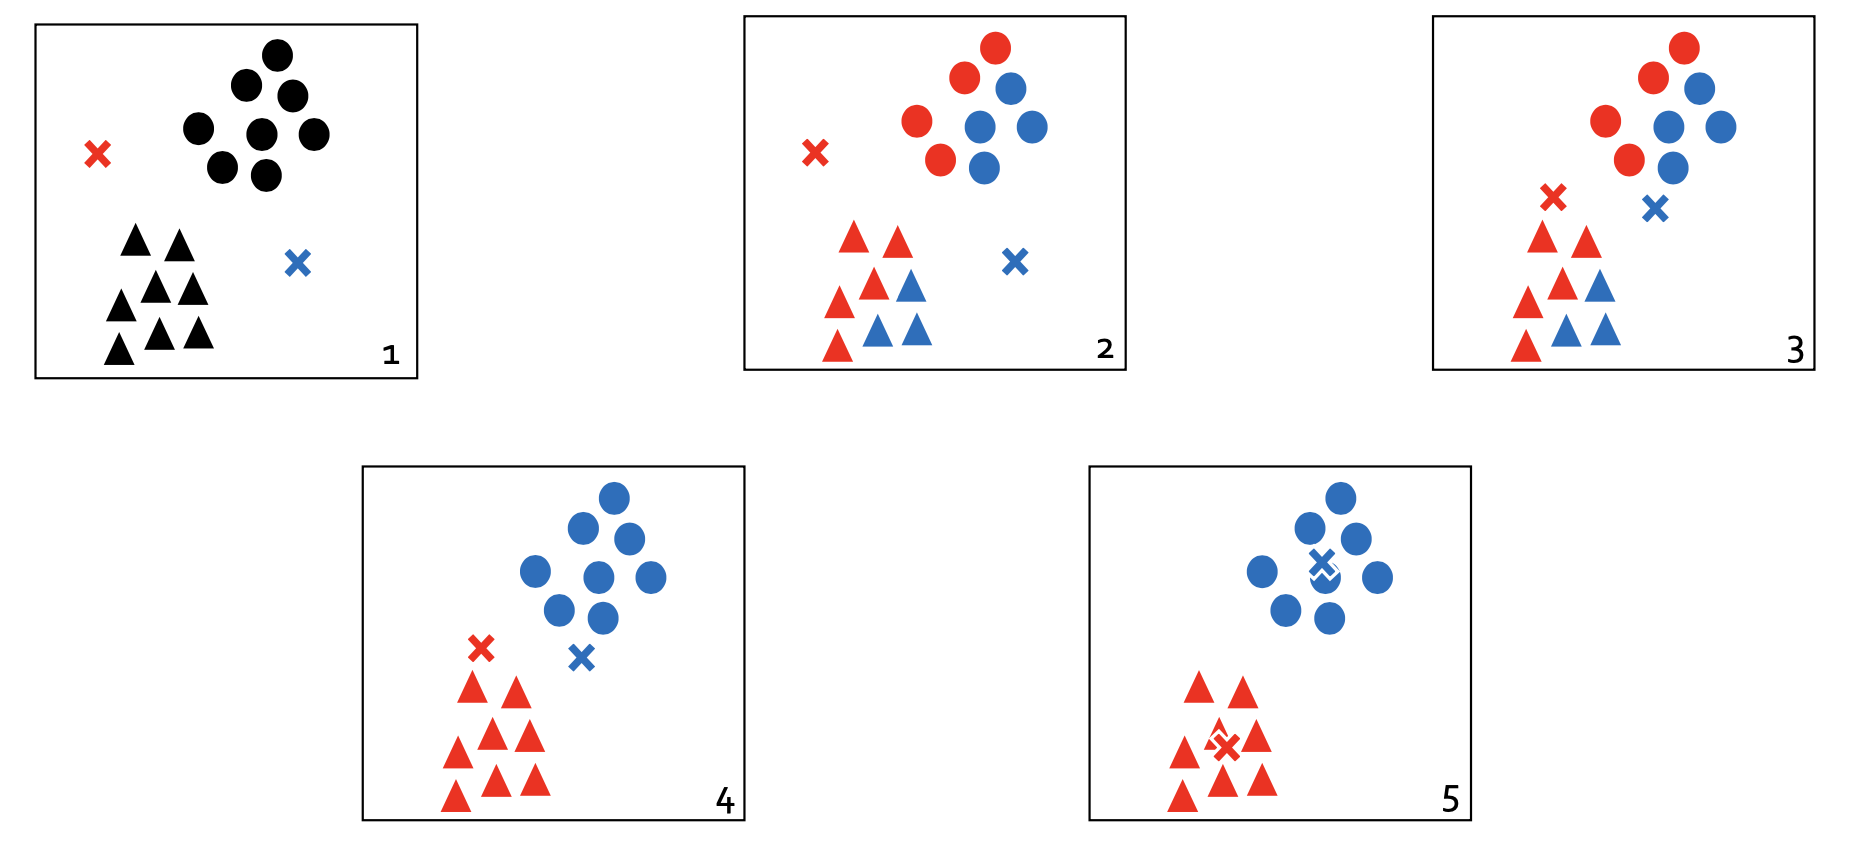
\includegraphics[width=0.5\textwidth]{./figures/chapter_7/lloydexample.png}
    \caption{K-Means algorithm}
    \label{fig:lloydex}
\end{figure}

The figure \ref{fig:lloydex} shows an example of the K-Means algorithm. The obtained clusters maybe are also optimal since the example was straightforward, but in general the algorithm may converge to a local minimum of the objective function.

\paragraph*{Convergence}
The nearest neighbor condition ensure us that when the cluster configurations changes, the cost $J$ will decrease or remain the same. So, $J$ is a \textit{monotonic} function of the cluster configuration.
But this is not sufficient to prove that the algorithm converges, because the algorithm may diverge to -$\infty$. However, sinche the objective function is bounded below by $0$ (because it is a squared sum) the algorithm must converge, at least to a local minimum.

Even if both the neighborhood condition and the centroid condition are satisfied, the algorithm may not converge to the global optimum. These two conditions are necessary but not sufficient for convergence to the global optimum.

% proof of necessary condition


In the last lecture, we've showed that the K-Means algorithm is guaranteed to converge to a local minimum of the objective function under the nearest neighbor condition and the centroid condition.

If we initialize the centroids in the right way, the algorithm will converge to the global minimum. However, if we initialize the centroids in the wrong way, the algorithm may converge to a local minimum. This is because there are different configurations of the centroids that satisfy the two conditions, but for us they are not equivalent.

% example 

Another thing is that the algorithm will converge in a finite number of steps, but the number of steps may be very large, due to the combinatorial nature of the problem. In practice, a commond stop criterion is that the algorithm is stopped when the change in the objective function is below a certain threshold.

\paragraph*{Initialization}
The performance of K-means in terms of \textit{clusters found} and \textit{convergence time} can be profoundly affected by the initialization we make of the centroids.

Random choice of $\mu_k$ is a very common and simple method, but not an optimal one. For example, choosing initial centroids far from observations can slow down the algorithm.

A popular initialization method, used in several software libraries, is the so-called \textbf{K-means++}. 
It uses probabilistic heuristics to choose initial centroids:

\begin{itemize}
    \item Centroids are selected randomly from data observations, but the probability with which they are chosen depends on the distance from the already selected centroids
    \item The farther a point is from a centroid, the higher the probability that this point is chosen as another centroid.
\end{itemize}


\section{Gaussian Mixture Model}
The Gaussian Mixture Model is a distribution-based clustering algorithm. The idea is that we assume that the observations have been generated by a mixture of $K$ Gaussian distributions, each of which is representative of a cluster. 
% The parameters of the model are estimated from the observations using an \textit{expectation-maximization} algorithm.

With $K$ clusters, the mixture model for the distribution of the entry $x_n$ is defined as:
\[
    p(x_n) = \sum_{k=1}^{K} \pi_k p_k (x_n \mid \theta_k)
\]
where the coefficients $\pi_k$ are called \textbf{mixing probabilities}, and they are constrained to be non-negative and to sum to $1$. The mixing probabilities are to be learned from the data.
These coefficients could be function of the number of observations in the cluster represented by the $k$-th Gaussian, but they are usually fixed to a constant value.

In the Gaussian Mixture Model, the individual likelihoods $p_k(\cdot \mid \theta_k)$ are $h$-dimensional multivariate Gaussian distributions, parametrized by the mean $\mu_k$ and the covariance matrix $\Sigma_k$:
\[
    p_k(x \mid \mu_k, \Sigma_k) = \frac{1}{(2\pi)^{\frac{h}{2}} \sqrt{\det \Sigma_k}} \exp{-\frac{1}{2}(x-\mu_k)^T \Sigma_k^{-1} (x-\mu_k)}
\]

\subsubsection*{Estimating the parameters}
The unknown parameters of the model are the mixing probabilities $\pi_k$, the means $\mu_k$ and the covariance matrices $\Sigma_k$ for $k=1, \ldots, K$.

\begin{figure}
    \centering
    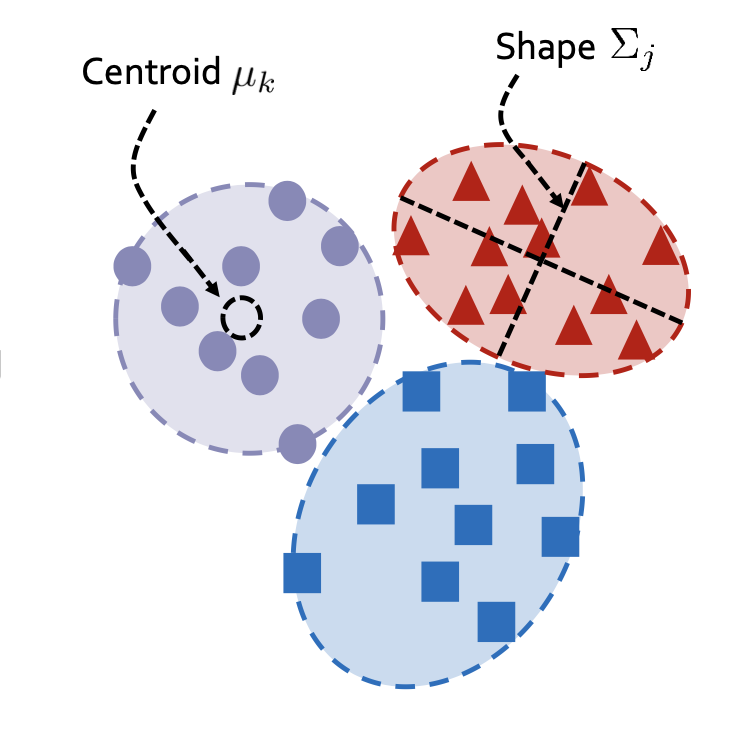
\includegraphics[width=0.5\textwidth]{./figures/chapter_7/gmmparam.png}
    \caption{Role of paramters in GMM}
    \label{fig:gmmparam}
\end{figure}

A solution could be to use the maximum likelihood estimator to estimate the parameters of the model by trying to maximize the log-likelihood function:
\[
    \log p(X \mid \pi, \mu, \Sigma) = \sum_{n=1}^{N} \log \left( \sum_{k=1}^{K} \pi_k p_k(x_n \mid \mu_k, \Sigma_k) \right)
\]

However, there is no closed form solution for the maximization, because all of the quantities we find depend on a term called \textbf{responsibility} $\gamma_{nk}$ that is not known and depends on the parameters on the model.
\[
    \gamma_{nk} = \frac{\pi_k p_k(x \mid \mu_k, \Sigma_k)}{\sum_{j=1}^{K} \pi_j p_j(x \mid \mu_j, \Sigma_j)}
\]
while the parameters can be computed as:
\[
    \pi_k = \frac{1}{N} \sum_{n=1}^{N} \gamma_{nk}
\]
\[
    \mu_k = \frac{\sum_{n=1}^{N} \gamma_{nk} x_n}{\sum_{n=1}^{N} \gamma_{nk}}
\]
\[
    \Sigma_k = \frac{\sum_{n=1}^{N} \gamma_{nk} (x_n - \mu_k)(x_n - \mu_k)^T}{\sum_{n=1}^{N} \gamma_{nk}}
\]
The paramters we called \textit{responsibilities} represents the posterior probabilities that the observation $x_n$ has been generated by the $k$-th Gaussian. In fact, they'are calculated in a similar way to the Bayes' rule.

\subsubsection*{Expectation-Maximization Algorithm}

From the previous formulation, we can see that we need an iterative algorithm to estimate the parameters of the model. For this reason, we use the \textbf{expectation-maximization} algorithm.

The basic idea of the algorithm is to estimate in an alternating manner the estimation of unknown coefficients and responsibilities by starting with an initial guess of the parameters.

\begin{algorithm}
    \SetAlgoLined
    Input: data set $X$, number of clusters $K$, initial parameters $\mu, \Sigma, \pi$ \\
    \Repeat{termination criterion is met}{
        Evaluate the log-likelihood with the current guess of paramters \\
        \textbf{Expectation step:} with the parameters fixed we compute the responsibility \\
        \textbf{Maximization step:} with the responsibilities fixed we compute the parameters and the new value of log-likelihood \\
    }
    \caption{EM algorithm for Gaussian Mixture Model}
\end{algorithm}

\begin{figure}
    \centering
    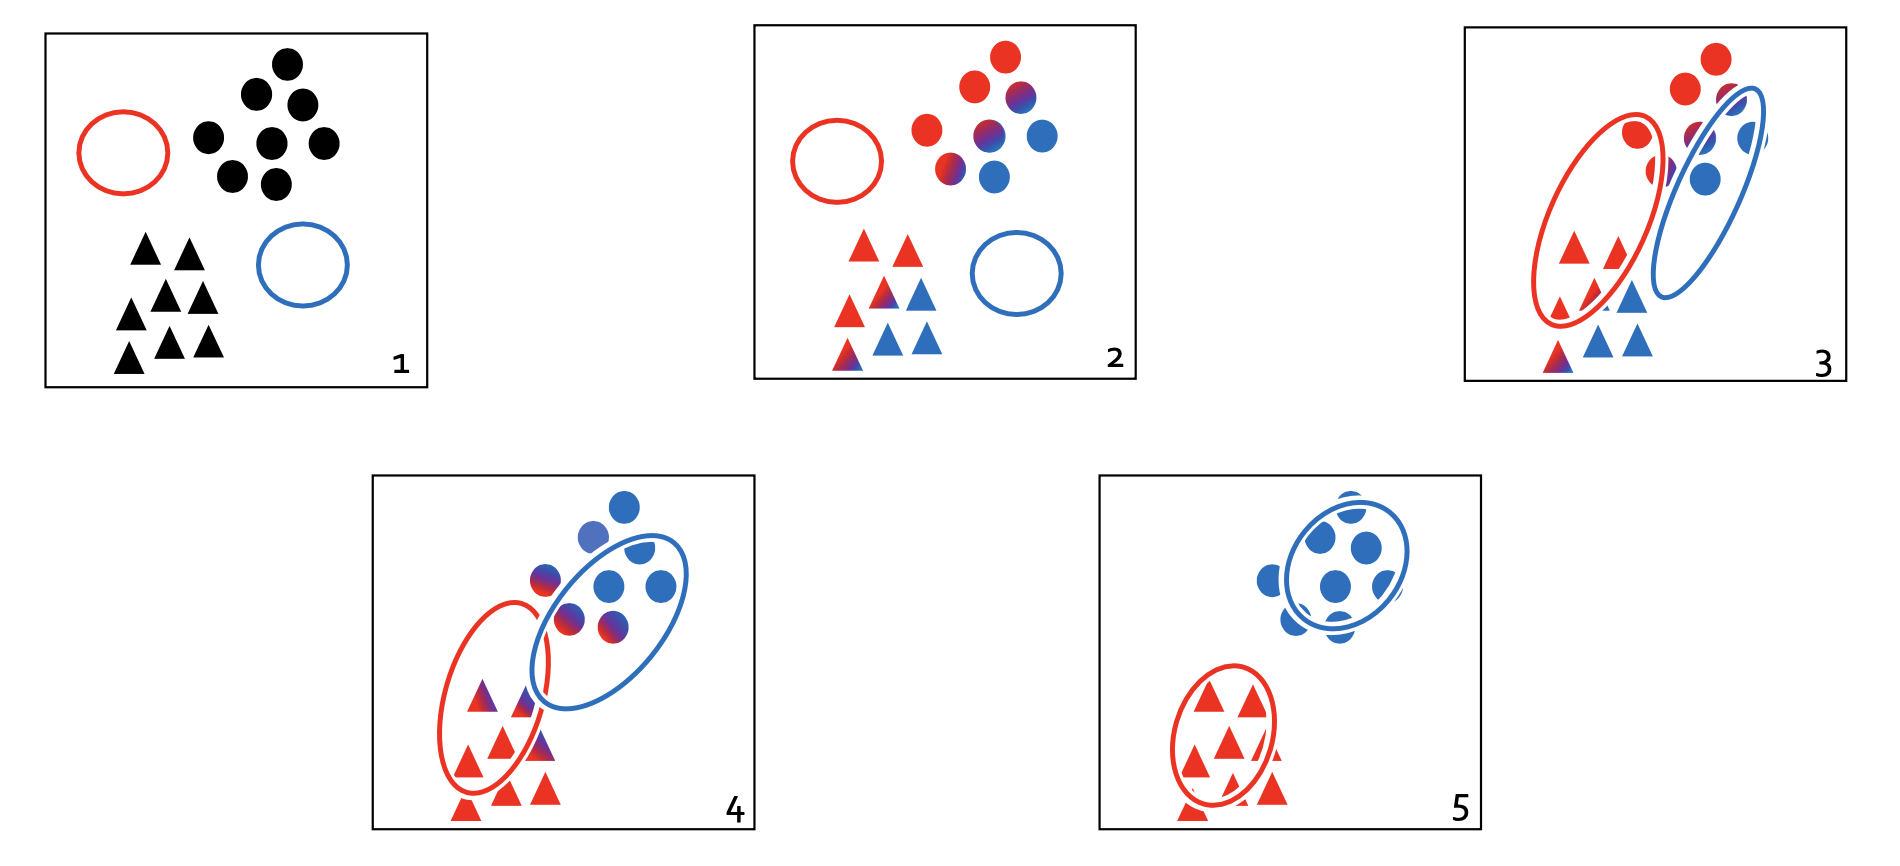
\includegraphics[width=0.5\textwidth]{./figures/chapter_7/emex.png}
    \caption{EM algorithm example}
    \label{fig:emex}
\end{figure}

In the plots of figure \ref{fig:emex}, however, since each data item has one probability of belonging to one Gaussian and one probability of belonging to another, we color them mixed.

The Expectation-Maximization algorithm is a general algorithm used not only in GMM clustering to find maximum likelihood solutions in problems where there are \textbf{latent variables}.

A latent variable is a variabile that cannot be observed directly, but it is useful to explain the observed data. In the case of the Gaussian Mixture Model, the latent variable is the Gaussian from which the observation has been generated.

The Expectation-Maximization algorithm actually maximizes a surrogate objective function which allows to maximize the likelihood function of interest, because in the expectation step it computes the expectation of the log-likelihood with respect to the conditional distribution of the latent variables given the observations, while the maximization step find the parameters that maximize the expectation and will then be used for the next expectation step.

\paragraph*{Convergence}
The convergence conditions are similar to the K-Means algorithm. EM is not guaranteed to converge to the global maximum of the likelhood, but it is guaranteed to increase the value of the likelihood function at each step.

\section{Hierarchical Clustering}
Hierarchical clustering can be performed in two ways: agglomerative or divisive.
We will focus on the \textbf{agglomerative clustering}, which starts from \textbf{singleton clusters}, that are the single data observations. At each step of the algorithm, the two most similar clusters are merged. There are different \textit{similarity measures} that we can use to find similar clusters.

By repeating the \textit{agglomeration process} we obtain a binary tree structure called \textbf{dendogram}, in which the root of this structure represents the entire dataset, while the leaves represent singleton clusters. Only by slicing the dendogram at a given height we obtain the cluster, this means that, differently from the other algorithms, $K$ is not an input of the algorithm but a parameter chosen by the user. $K$ depends on the specific application domain.

\subsubsection{Similarity Measures}

\begin{algorithm}
    \SetAlgoLined
    Input: data set $X$ \\
    \Repeat{One single cluster remains}{
        Examine all pairs of subgroups, and merge the most similar \\
    }
    \caption{Agglomerative Clustering}
\end{algorithm}

The dissimilarity $d(G,H)$ between two groups of observations $G$ and $H$ is computed from the pairwise dissimilarities $d_{ii^{\prime}}$ between the observations in the two groups. There are different ways to compute the dissimilarity between two groups:
\begin{itemize}
    \item \textbf{Single-linkage}
    \item \textbf{Complete-linkage}
    \item \textbf{Group average}
    \item \textbf{Ward's criterion}
\end{itemize}

\paragraph*{Single Linkage}
The single linkage measure is defined as:
\[
    d_{SL}(G,H) = \min_{i \in G, i^{\prime} \in H} d_{ii^{\prime}}
\]

The similarity among subgroups is based on the similarity between the \textbf{nearest observations}. This method tends to produce \textbf{elongated clusters}, with non-elliptical shapes and it is sensitive to noise and outliers.

An explanation of the single linkage is shown in figure \ref{fig:singlelinkage}.
\begin{figure}[h]
    \centering
    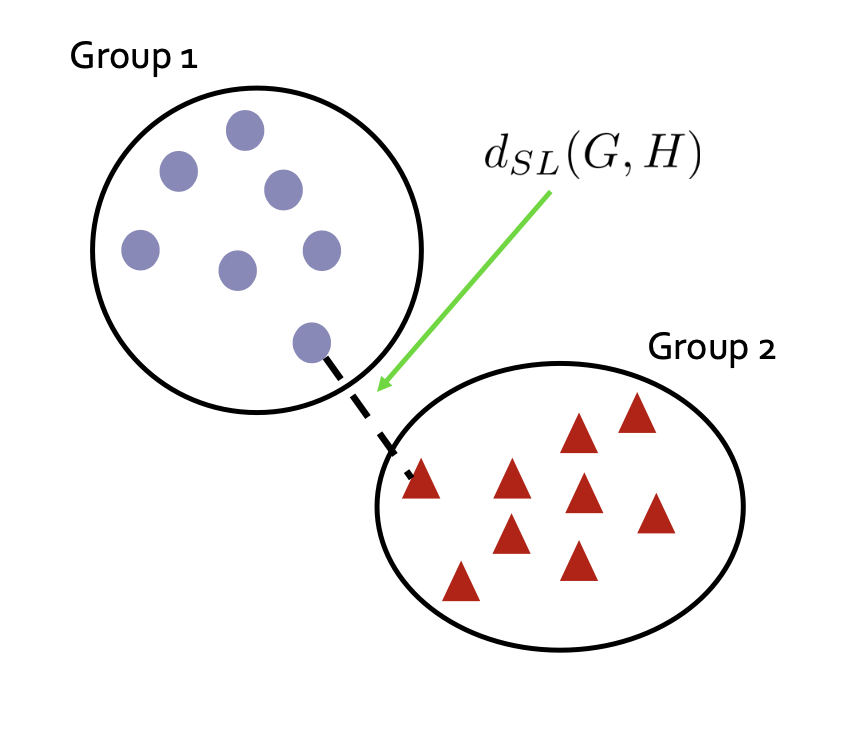
\includegraphics[width=0.5\textwidth]{./figures/chapter_7/singlelinkage.png}
    \caption{Single linkage explanation}
    \label{fig:singlelinkage}
\end{figure}

\paragraph*{Complete Linkage}
The complete linkage measure is defined as:
\[
    d_{CL}(G,H) = \max_{i \in G, i^{\prime} \in H} d_{ii^{\prime}}
\]

The similarity among subgroups is based on the similarity between the \textbf{farthest observations}. This method tends to produce compact clusters, because it merges the smallest diameter clusters first. It is still sensitive to noise and outliers.

\paragraph*{Average Group}
The average group measure is defined as:
\[
    d_{GA}(G,H) = \frac{1}{N_G N_H} \sum_{i \in G} \sum_{i^{\prime} \in H} d_{ii^{\prime}}
\]
Where $N_G$ and $N_H$ are the number of observations in the groups $G$ and $H$ respectively.

The similarity among subgroups is based on the average similarity between the "centroid" of the groups. This methods is in between the single and complete linkage.

An explanation of the average group is shown in figure \ref{fig:averagegroup}.
\begin{figure}[h]
    \centering
    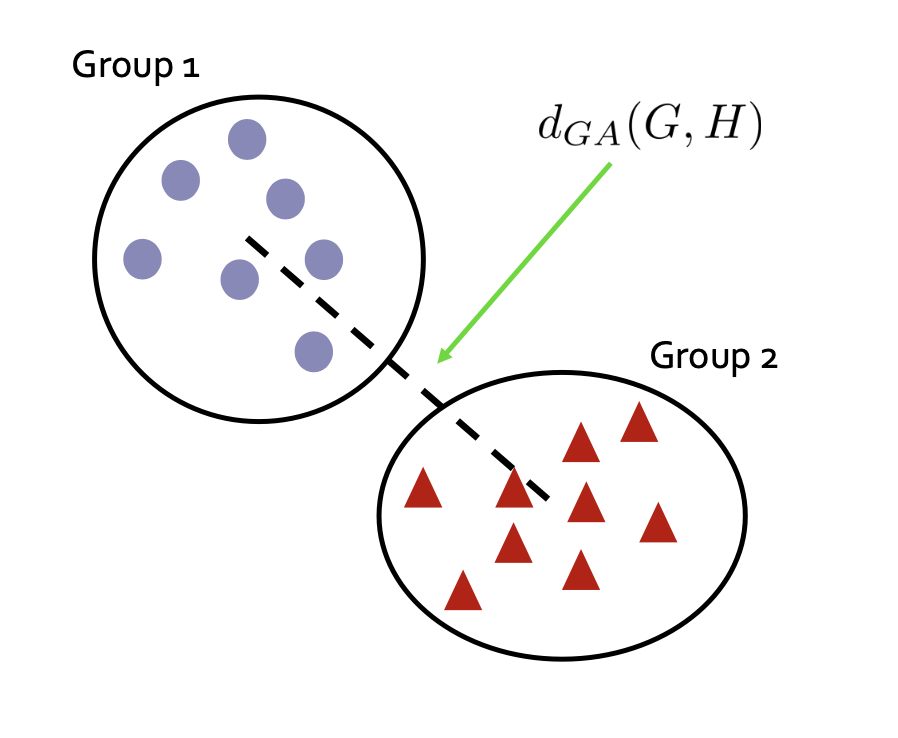
\includegraphics[width=0.5\textwidth]{./figures/chapter_7/averagegroup.png}
    \caption{Average group explanation}
    \label{fig:averagegroup}
\end{figure}

\paragraph*{Ward's Criterion}
Ward's criterion is defined as:
\[
    d_W(G,H) = \frac{N_G N_H}{N_G + N_H} \| \mu_G - \mu_H \|^2
\]
where $\mu_G$ and $\mu_H$ are the centroids of the groups $G$ and $H$ respectively.

It can be shown that this method is equivalent to measuring the increase of variance when merging two groups.

An explanation of Ward's criterion is shown in figure \ref{fig:wardcriterion}.
\begin{figure}[h]
    \centering
    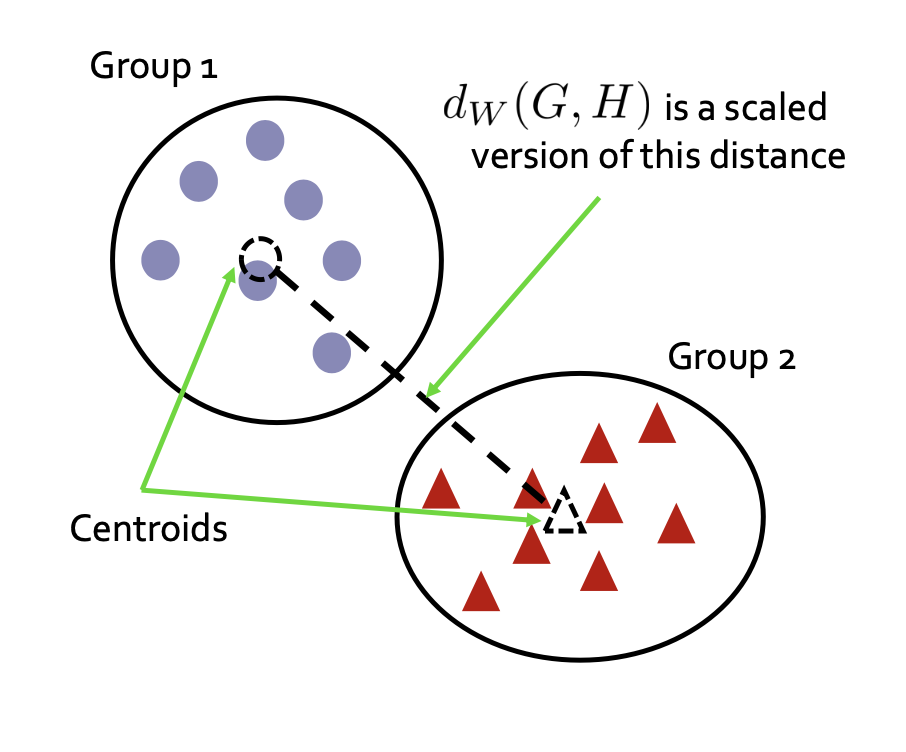
\includegraphics[width=0.5\textwidth]{./figures/chapter_7/wardcriterion.png}
    \caption{Ward's criterion explanation}
    \label{fig:wardcriterion}
\end{figure}

\paragraph*{Choosing the number of clusters}
To choose the number of clusters, there are different \textit{heuristics} scores that can be used:
\begin{itemize}
    \item \textbf{Silhouette score}
    \item \textbf{Caliniski-Harabasz score}
\end{itemize}

\subparagraph*{Silhouette Score}
The \textbf{silhoutte coefficient} evaluates how similar the observations to one cluster are to others.

Let $a(n)$ be the average distance between data $x_n$ and other points in its cluster, and let $b(n)$ be the average distance between $x_n$ and all other points.

The coefficient is the quantity $s(n)\in[-1,1]$ defined as

\[
    s(n)=\frac{b(n)-a(n)}{\max\{a(n),b(n)\}}
\]

Such a quantity will be:
\begin{itemize}
    \item Close to $1$ for good matching of $x_n$ to its cluster
    \item Small or negative for a bad matching of $x_n$ to its cluster
\end{itemize}

Averaging these coefficients for all observations we obtain a \textbf{silhoutte score} associated with the number of clusters $K$. 

Repeating the procedure for several $K$ we go to choose the one with the largest silhoutte score.
\subparagraph*{Caliniski-Harabasz score}

Let be the \textbf{between cluster variance}

\[
    B(K)=\sum_{k=1}^KN_k\|\mu_k-\mu\|^2
\]

Where:
\begin{itemize}
    \item $N_k$ is the number of points in the cluster $k$
    \item $\mu_k$ is the centroid of the cluster $k$
    \item $\mu$ is the centroid of the entire dataset.
\end{itemize}

Let be the \textbf{within cluster variance}
\[
    W(K)=\sum_{k=1}^K\sum_{x\in C_k}\|x-\mu_k\|^2
\]

The \textbf{Calinski-Harabasz score} is defined as.

\[
    \frac{B(K)}{W(K)}\frac{N-K}{K-1}
\]

A high value indicates that the clusters are \textit{dense and well separated}.

Again, the number of clusters $K$ is the one with which the highest score value is associated.

\section{DBSCAN}
\textbf{DBSCAN} segments observations by examining \textit{dense} regions with a given \textit{reachability}.

\begin{itemize}
    \item The \textbf{density} is estimated by counting the number of observations that fall within a of predetermined radius.
    \item The \textbf{reachability} is based on connecting a data observation to a dense region. 
\end{itemize}

Although DBSCAN does not require the number of clusters a priori, it still relies on two fundamental parameters:
\begin{itemize}
    \item $\epsilon$, which is the \textit{radius} of the neighbourhood considered to detect density
    \item $minPts$, which represents the minimum number of points that must fall within the $\epsilon$ radius
\end{itemize}

To verify if a point fall within the $\epsilon$ radius, the algorithm still use a distance measure, such as the Euclidean distance.

\subsubsection*{Base concepts}
A \textbf{core point} $p$ is an observation whose $\epsilon$-neighbouhood contains at least $minPts$ observations ($p$ included).

A point $q$ is \textbf{directly density-reachable} from a core point $p$ if $q$ lies in the $\epsilon$-neighbourhood of $p$.

A point $p$ is \textbf{density-reachable} from $q$ if there exists a chain of points $p_1,\dots,p_n$, where $p_1=p$ and $p_n=q$, such that the point $p_{i+1}$ is \textit{directly density-reachable} from $p_i$.

A point $p$ is \textbf{density-connected} to a point $q$ if there is a point $o$ such that both $p$ and $q$ are \textit{directly density reachable} from $o$.

\begin{figure}
    \centering
    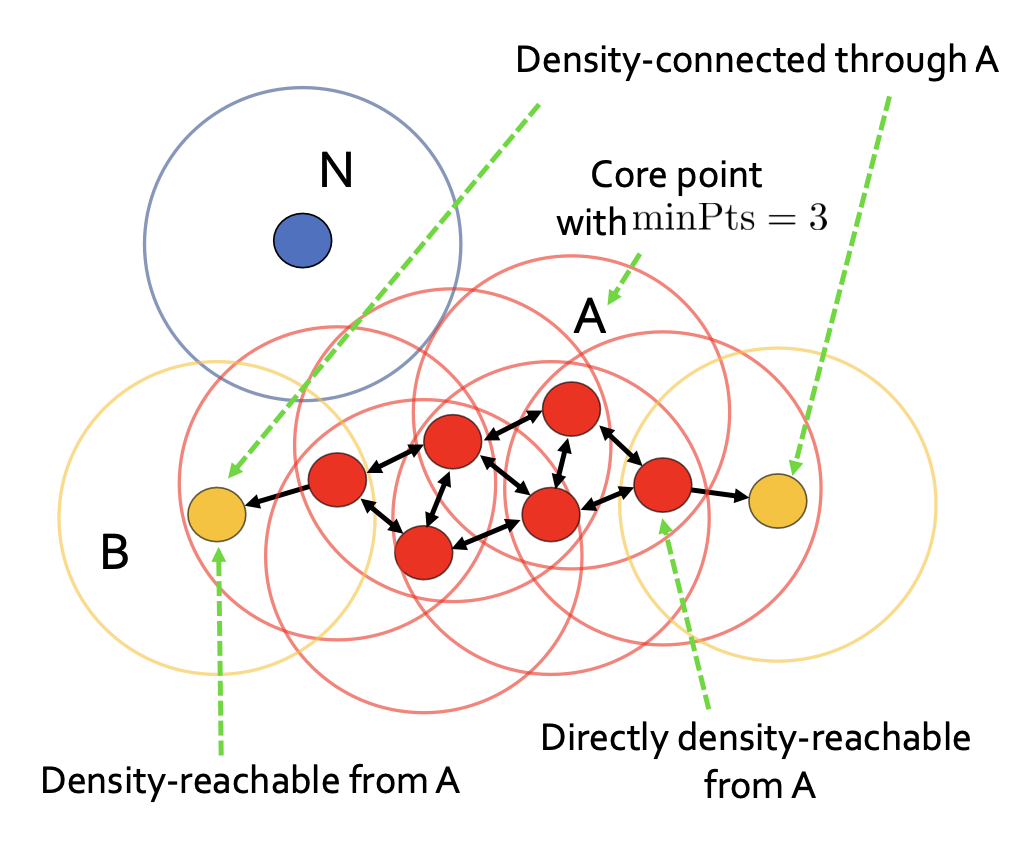
\includegraphics[width=0.5\textwidth]{./figures/chapter_7/dbscanconcepts.png}
    \caption{DBSCAN concepts}
    \label{fig:dbscan}
\end{figure}

\subsubsection*{DBSCAN clusters}
A \textbf{density-based cluster} is a nonempty set of observations such that:

\begin{itemize}
    \item If a point $p$ belongs to the cluster and $q$ is a \textit{density-reachable} point from $p$, then $q$ belongs to the cluster
    \item If points $p$ and $q$ belong to the same cluster, then they must be \textit{density-connected}
\end{itemize}

There may be observations that do not belong to any cluster; such points are called \textbf{noise points}.

Observations that belong to a cluster but do not have a dense neihbourhood are called \textbf{border points}.

\begin{figure}
    \centering
    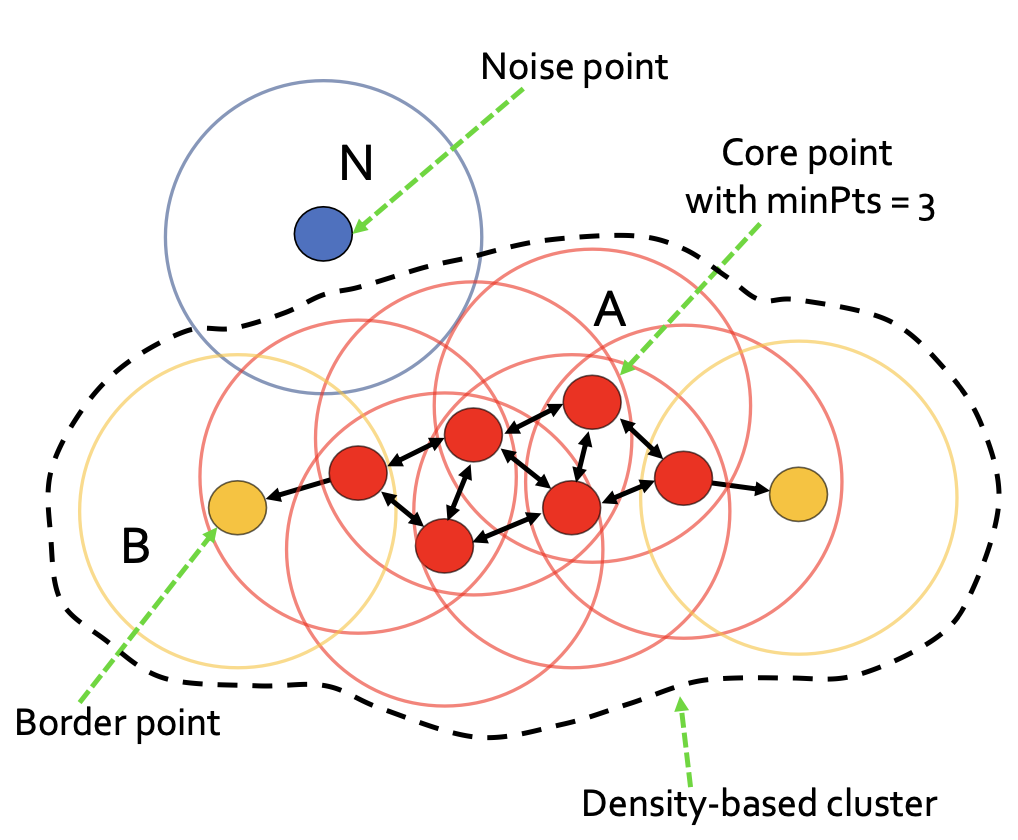
\includegraphics[width=0.5\textwidth]{./figures/chapter_7/dbscanconcepts2.png}
    \caption{DBSCAN clusters}
    \label{fig:dbscanclusters}
\end{figure}

\subsubsection*{Algorithm}
A pseudocode of the DBSCAN algorithm is shown in Algorithm \ref{alg:dbscan}.

\begin{algorithm}
    \SetAlgoLined
    Input: data set $D$, radius $\epsilon$, minimum number of points $minPts$ \\
    \For{each point $p$ in $D$}{
        \If{$p$ has been already assigned to a cluster}{
                \textbf{continue}
            }
        Get the $\epsilon$-neighbourhood $ N (p, \epsilon)$ of $p$ \\
        \If{the number of points in $ N (p, \epsilon)$ is less than $minPts$}{
            Assign $p$ as a \textbf{noise point} \\
            \textbf{continue}
        }
        Start a new cluster $C$ \\
        Assign $p$ to $C$ \\
        Compute $S= N(p,\epsilon) \backslash \{p\}$ \\
        \For{each point $q$ in $S$}{
            \If{$q$ is a \textit{noise point}}{
                assign $q$ to $C$
                }
            \If{$q$ has been already assigned to a cluster}{
                \textbf{continue}
                }
            Get the $\epsilon$-neighbourhood $ N (q, \epsilon)$ of $q$ \\
            Assign $q$ to $C$ \\
            \If{the number of points in $ N (p, \epsilon)$ is less than $minPts$}{
                \textbf{continue}
                }
            $S = S \cup  N (q, \epsilon)$
        }
    }
    \caption{DBSCAN algorithm}
    \label{alg:dbscan}
\end{algorithm}